\vspace{-3em}

\begin{IEEEbiography}
    [{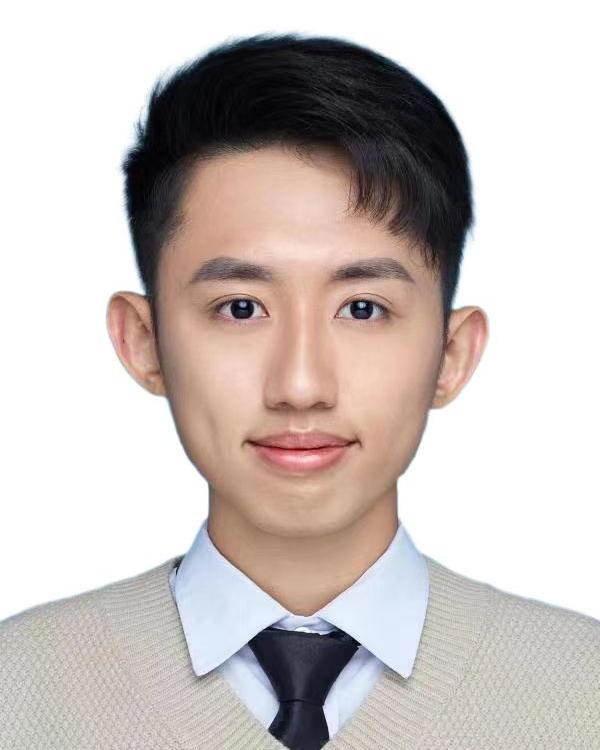
\includegraphics[width=1in,height=1.25in,clip,keepaspectratio]{Figs_bio/JunjieHe.jpg}}]
    {Junjie He} received the B.E. degree in Automation from Guangdong University of Technology, in 2022, and the M.E. degree in artificial intelligence from Xi’an Jiaotong University, in 2025. He is currently pursuing the Ph.D. degree with the Thrust of Robotics and Autonomous Systems, The Hong Kong University of Science and Technology (Guangzhou). His research interests include world models, robotic manipulation, and 3D/4D generation.
\end{IEEEbiography}

\vspace{-3em}

\begin{IEEEbiography}
    [{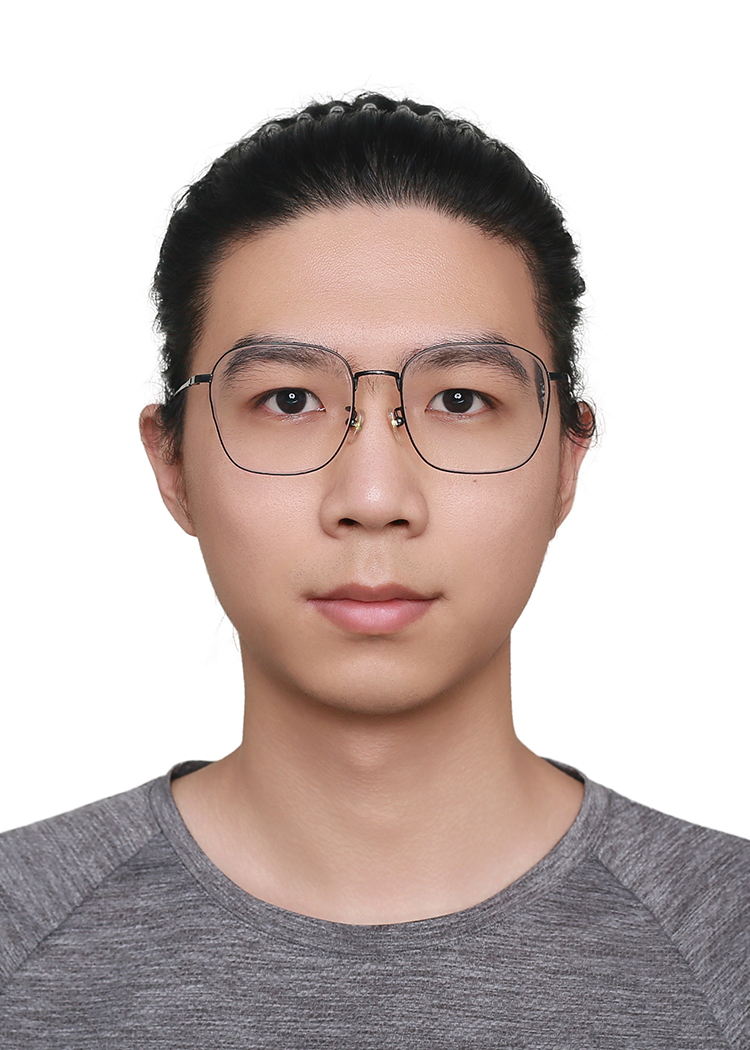
\includegraphics[width=1in,height=1.25in,clip,keepaspectratio]{Figs_bio/JunfengLi.jpg}}]
    {Junfeng Li} received the B.E. degree in Mechanical Engineering from the University of Birmingham and Wuhan University of Technology in 2021, and the M.S. degree in Computer Science from University College London in 2023. From 2024 to 2025, he was a Research Assistant with the Thrust of Robotics and Autonomous Systems, The Hong Kong University of Science and Technology (Guangzhou). He is currently pursuing the Ph.D. degree with the Thrust of Intelligent Transportation, The Hong Kong University of Science and Technology (Guangzhou). His research interests include 3D computer vision and 3D/4D generation.
\end{IEEEbiography}

\vspace{-3em}

\begin{IEEEbiography}
    [{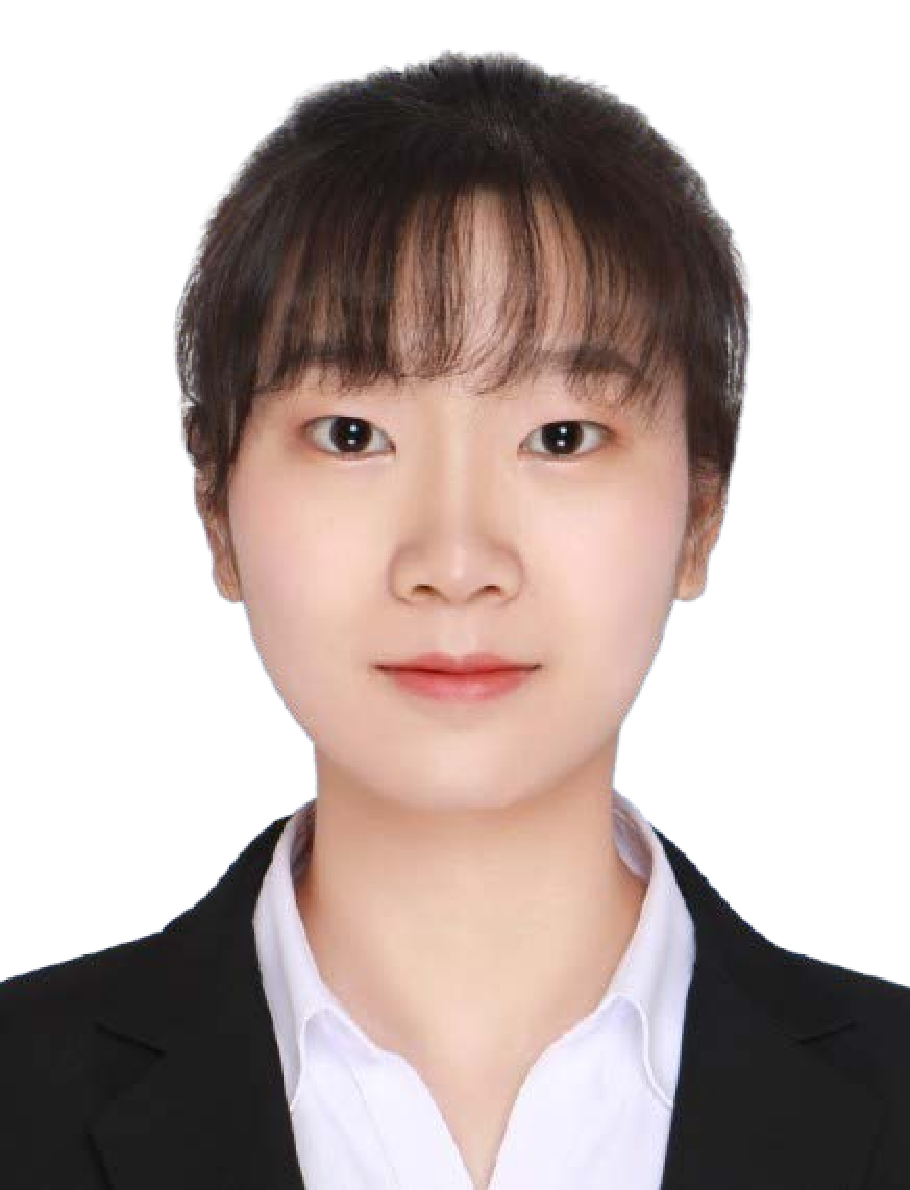
\includegraphics[width=1in,height=1.25in,clip,keepaspectratio]{Figs_bio/WenjieLiu.pdf}}]
    {Wenjie Liu} received the B.E. degree in computer science and technology from Xi’an University of Technology, in 2021, and the M.E. degree in software engineering from Northwestern Polytechnical University, in 2024. Since 2024, she has been a Research Assistant with the Thrust of Robotics and Autonomous Systems, The Hong Kong University of Science and Technology (Guangzhou). Her research interests include 2D/3D computer vision and 2D/3D generation.
\end{IEEEbiography}

\vspace{-3em}

\begin{IEEEbiography}
    [{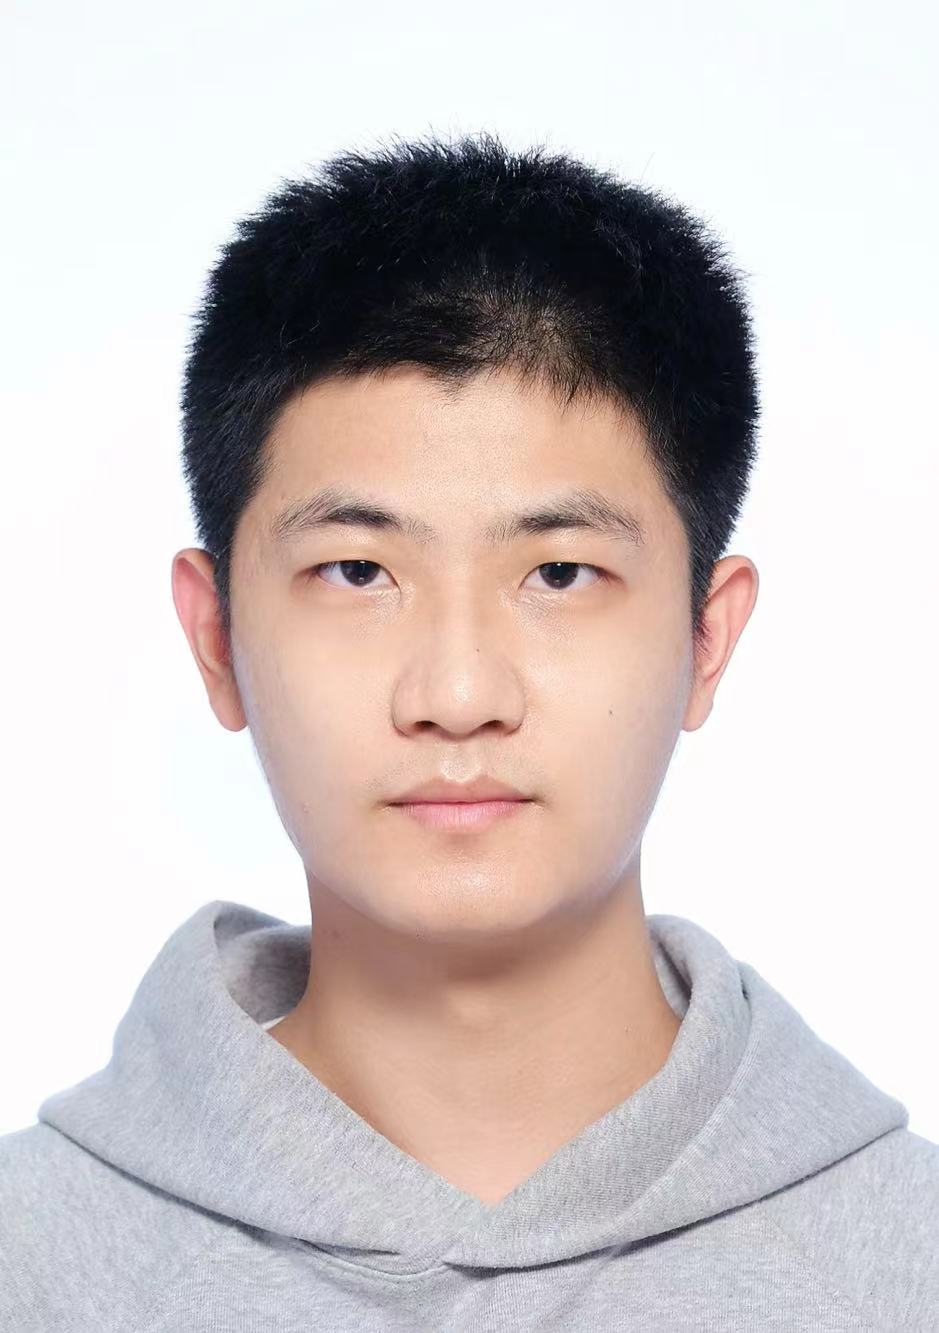
\includegraphics[width=1in,height=1.25in,clip,keepaspectratio]{Figs_bio/TianyuHuang.jpg}}]
    {Tianyu Huang} received the B.E. degree from the College of Optical Science and Engineering, Zhejiang University, Zhejiang, China in 2020 and the Ph.D. degree in the Department of Mechanical and Automation Engineering, The Chinese University of Hong Kong, Hong Kong in 2024. He is currently a postdoctoral researcher with the Hong Kong Centre for Logistics Robotics, The Chinese University of Hong Kong. His research interests lie in 3D robot perception, robot manipulation, and optimization.
\end{IEEEbiography}

\vspace{-3em}

\begin{IEEEbiography}
    [{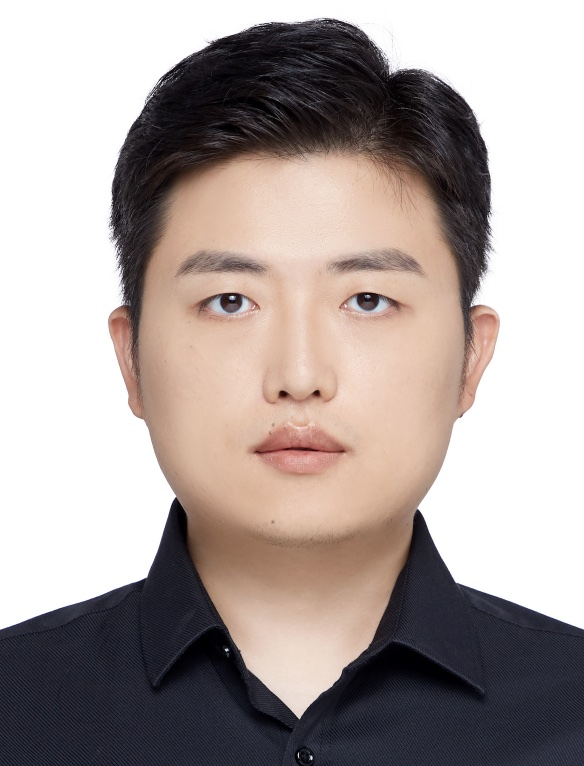
\includegraphics[width=1in,height=1.25in,clip,keepaspectratio]{Figs_bio/ShunboZhou.jpg}}]
    {Shunbo Zhou} received the B.Eng. degree in instrument science and technology from China Jiliang University, Hangzhou, China, in 2014, and the Ph.D. degree in mechanical and automation engineering from The Chinese University of Hong Kong, Shatin, Hong Kong, in 2020.
    He is currently a joint post-doctoral research fellow at HKCLR and CUHK Robotics Institute (CURI). 
    % He is also leading the Mobile Robotics Group of HKCLR and CURI to develop 
    His research interests include 
    autonomous robots/vehicles and related technologies for logistics and mine applications.
\end{IEEEbiography}

\vspace{-3em}

\begin{IEEEbiography}
    [{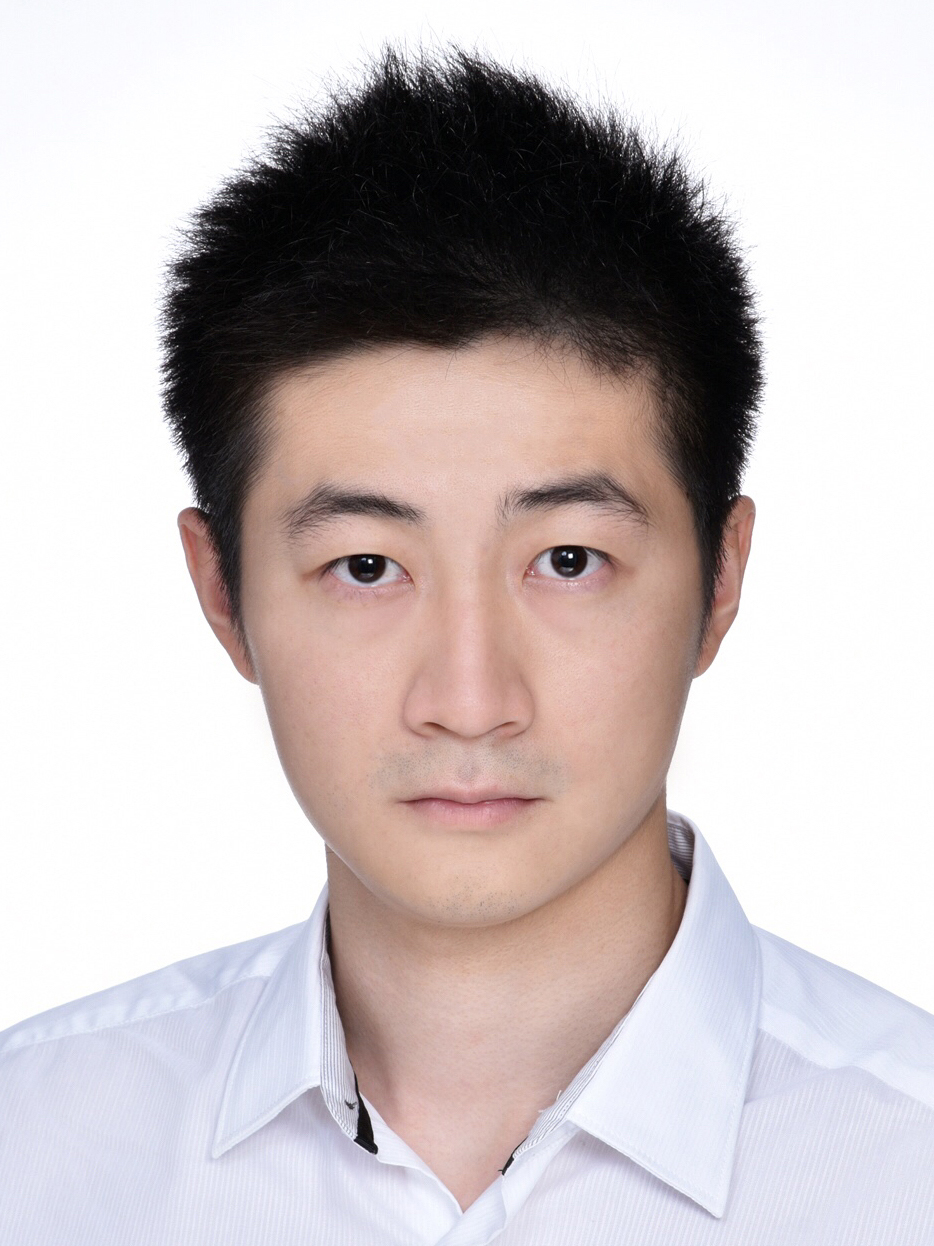
\includegraphics[width=1in,height=1.25in,clip,keepaspectratio]{Figs_bio/junma.jpg}}]
    {Jun Ma} received the B.Eng. degree with First Class Honours in electrical and electronic engineering from Nanyang Technological University, Singapore, in 2014, and the Ph.D. degree in electrical and computer engineering from the National University of Singapore, Singapore, in 2018. From 2018 to 2021, he held several positions at the National University of Singapore; University College London, London, U.K.; University of California, Berkeley, Berkeley, CA, USA; and Harvard University, Cambridge, MA, USA. He is currently an Assistant Professor with the Robotics and Autonomous Systems Thrust, The Hong Kong University of Science and Technology (Guangzhou), Guangzhou, China.
    % , and also with the Division of Emerging Interdisciplinary Areas, The Hong Kong University of Science and Technology, Hong Kong SAR, China. 
    % He is also the Director of the Intelligent Autonomous Driving Center, The Hong Kong University of Science and Technology (Guangzhou). 
    His research interests include motion planning and control for robotics and autonomous driving.
\end{IEEEbiography}

\vspace{-3em}

\begin{IEEEbiography}
    [{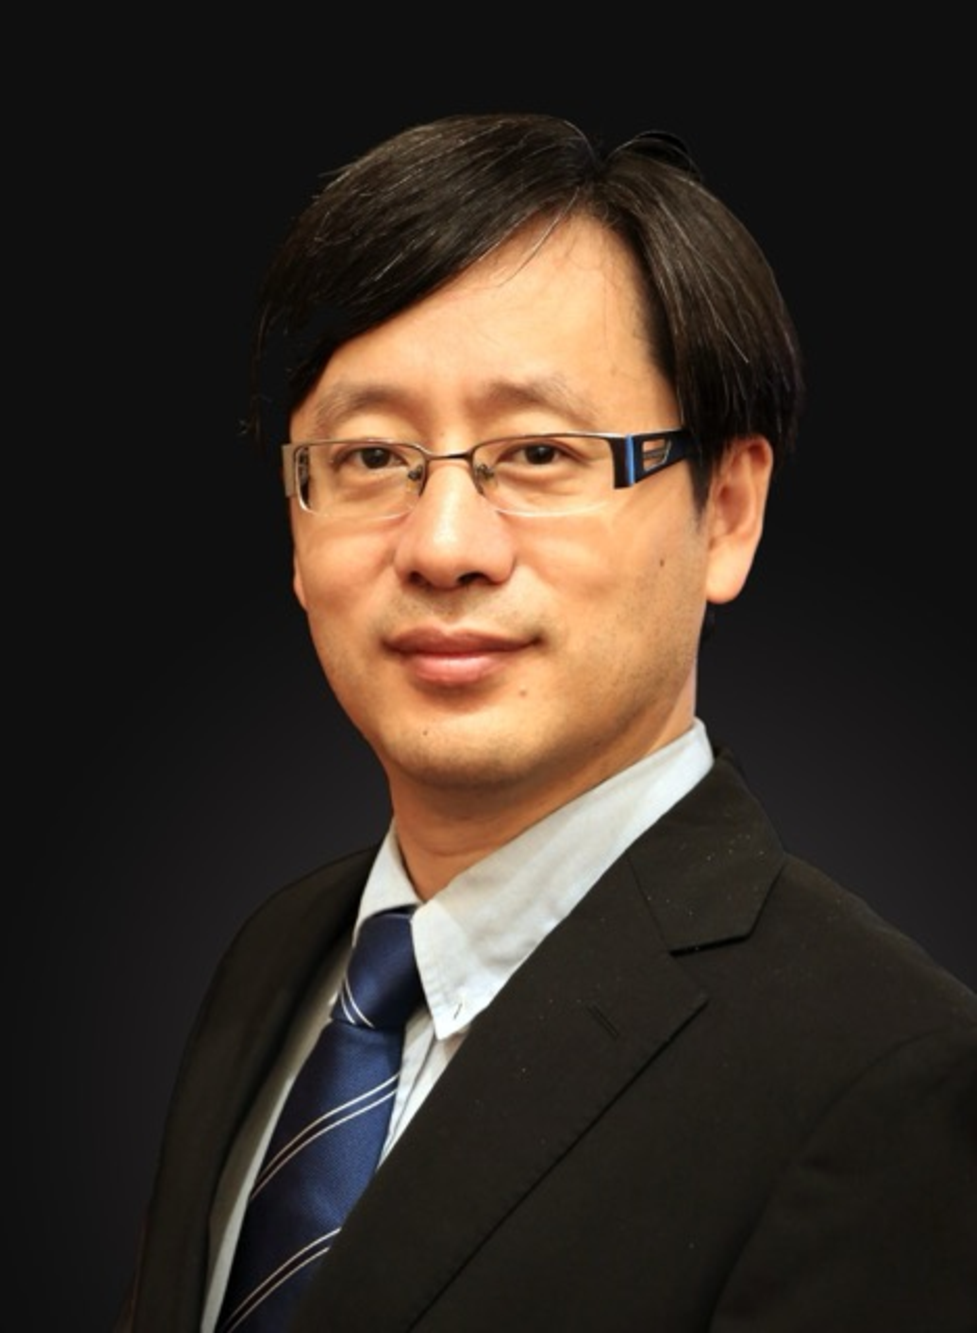
\includegraphics[width=1in,height=1.25in,clip,keepaspectratio]{Figs_bio/HeshengWang.pdf}}]
    {Hesheng Wang} received the B.Eng. degree in electrical engineering from the Harbin Institute of Technology, Harbin, China, in 2002, and the M.Phil. and Ph.D. degrees in automation and computer-aided engineering from The Chinese University of Hong Kong, Hong Kong, in 2004 and 2007, respectively. He is currently a Professor with the Department of Automation, Shanghai Jiao Tong University, Shanghai, China. His research interests include visual servoing, service robot, computer vision, and autonomous driving.
    He is a Senior Editor of the IEEE/ASME Transactions on Mechatronics, an Associate Editor of IEEE Transactions on Automation Science and Engineering, IEEE Robotics and Automation Letters, an Editor of Conference Editorial Board of IEEE Robotics and Automation Society. He served as an Associate Editor of the IEEE Transactions on Robotics from 2015 to 2019. 
    He is the General Chair of IEEE/RSJ IROS 2025.
\end{IEEEbiography}

\vspace{-4em} 

\begin{IEEEbiography}
    [{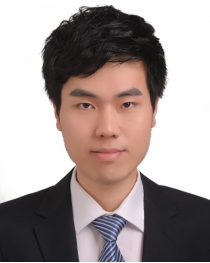
\includegraphics[width=1in,height=1.25in,clip,keepaspectratio]{Figs_bio/HaoangLi.pdf}}]
    {Haoang Li} received the B.E. and M.E. degrees in Remote Sensing and Information Engineering from Wuhan University, China, in 2016 and 2018, respectively, and the Ph.D. degree in Mechanical and Automation Engineering from The Chinese University of Hong Kong, Hong Kong, in 2022. He is currently an Assistant Professor of the Robotics and Autonomous Systems Thrust, and Intelligent Transportation Thrust,
    Hong Kong University of Science and Technology (Guangzhou), China.
    He was a Postdoc researcher with the Department of Informatics, Technical University of Munich, Germany from 2022 to 2024. He was a visiting PhD student with the Department of Computer Science, ETH Zurich, Switzerland, in 2021. His research interests include computer vision and robotics. His work was selected as CVPR 2025 Best Paper Award Candidate. He serves as an Associate Editor of ICRA and a Registration Chair of IROS 2025.
\end{IEEEbiography}